\section{Transmission Lines}
A transmission line is a special structure designed to guide waves. The waves are guided in a dielectric by means of reflections between the conductors.

\begin{itemize}
	\item TEM Modes: The direction of propagation is orthogonal to the direction of electric and magnetic field.
	\item TE Modes: The direction of propagation is normal to the E-field but not H-field.
	\item TM Modes: The direction of propagation is normal to the H-field but not E-field.
\end{itemize}


\subsection{Transmission Line Equations}
\begin{tabular}{p{8cm}p{4.5cm}p{5cm}}
	\begin{minipage}{8cm}
		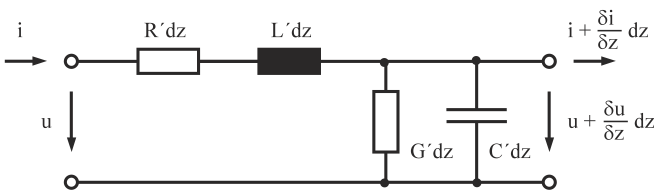
\includegraphics[width=8cm]{./images/LeitungselementESB.png}
	\end{minipage}&
	\begin{minipage}{4.5cm}
		\textbf{Distributed Parameters}\\
		$R'[\frac{\Omega}{m}]: \text{Resistance}$\\
		$L'[\frac{H}{m}]: \text{Inductance}$\\
		$G'[\frac{S}{m}]: \text{Conductance}$\\
		$C'[\frac{F}{m}]: \text{Capacity}$\\
	\end{minipage}&
	\begin{minipage}{5cm}
		\textbf{No Load}:\\
		$\underline{Y}_L=\frac{1}{\underline{Z}_L}=\frac{\underline{I}_L}
		{U} = G+j\omega C=\frac{\alpha l+j\beta l}{\underline{Z}_W}$\\
		\textbf{Short Circuit}:\\
		$\underline{Z_K}=\frac{U}{\underline{I}_K} = R+j\omega
		L=(\alpha l+j\beta l)\underline{Z}_W$\\
	\end{minipage}\\
	\begin{minipage}{8cm}
		\vspace{0.3cm}
		$\underline{U}_1=\cosh(\gamma l)\cdot \underline{U}_2+
		\underline{Z}_W \cdot \sinh(\gamma l)\cdot \underline{I}_2$\\
		$\underline{I}_1=\frac{1}{\underline{Z}_W}\cdot \sinh(\gamma l)\cdot
		\underline{U}_2+ \cosh(\gamma l)\cdot \underline{I}_2$  	
	\end{minipage} &
	\begin{minipage}{9cm}
		\vspace{0.3cm}
		$\begin{bmatrix}
		\underline{U}_1\\
		\underline{I}_1
		\end{bmatrix}=
		\begin{bmatrix}
		cosh(\gamma l) & \underline{Z}_W sinh(\gamma l)\\
		\frac{1}{\underline{Z}_W}sinh(\gamma l) & cosh(\gamma l)
		\end{bmatrix} \cdot
		\begin{bmatrix}
		\underline{U}_2\\
		\underline{I}_2
		\end{bmatrix}$\\
	\end{minipage}
\end{tabular}\\
if $\alpha l >> \beta l$ then $cosh(\gamma l)\approx sinh(\gamma
l)=\frac{1}{2} e^{\gamma l}$ !!!

\subsubsection{Lossy Transmission Lines}
\renewcommand{\arraystretch}{1.5}
\begin{tabular}{| p{7.7cm} | l |}
	\hline
	\textbf{Propagation Factor}
	& $\gamma=\alpha+j\beta=\sqrt{(R'+j\omega L')(G'+j\omega C')}\qquad
	\alpha=[\frac{Np}{m}] \qquad \beta=[\frac{^\circ}{m}]$\\
	\hline
	\textbf{Damping Constant}
	& $\alpha l= \frac{1}{2}ln(Re\{e^{2\gamma l}\})=\alpha\cdot l$\\
	\hline
	\textbf{Phase Delay}
	& $\beta l=\frac{1}{2}ln(Im\{e^{2\gamma l}\})= \beta\cdot l$ \qquad
	$\beta=\frac{\omega}{v_P}$\\
	\hline
	\textbf{Characteristic Impedance}
	& $\underline{Z}_W=\frac{\underline{U}}{\underline{I}}=\sqrt{\frac{R'+j\omega L'}{G'+j\omega C'}}$
	$=\sqrt{\underline{Z}_L \cdot \underline{Z}_K}$\\
	\hline
	\textbf{Input Imp. $\underline{Z}_1$  with termination $\underline{Z}_a$} &
	$\underline{Z}_1 = \underline{Z}_W
	\frac{\underline{Z}_a+\underline{Z}_W \cdot \tanh(\gamma
		l)}{\underline{Z}_W+\underline{Z}_a \cdot \tanh(\gamma l)}
	= \underline{Z}_W \frac{e^{+j \gamma l} + \underline{\Gamma}_{Last} e^{- j \gamma l}}
	{e^{+j \gamma l} - \underline{\Gamma}_{Last} e^{- j \gamma l}}$\\
	\hline
	\textbf{Phase Velocity, Wave length}
	& $v_P=\frac{1}{\sqrt{L'C'}}=\frac{\lambda}{T}$ \qquad
	\qquad $\lambda=\frac{2\pi}{\beta}=\frac{v_P}{f} \approx
	\lambda=\frac{\lambda_0}{\sqrt{\varepsilon_r \mu_r}} \quad \beta=[rad]$\\
	\hline
	\textbf{Free space Wave Length}
	& $\lambda_0=\frac{c}{f}=\frac{2\pi c}{\omega} \qquad c\approx 3*10^8 \frac{m}{s}$\\
	\hline
	\textbf{Wave Equations}
	& $\begin{matrix}
	\underline{U}(z)=\underline{U}^+_0 \cdot e^{-\gamma z} + \underline{U}^-_0 \cdot e^{\gamma z}\\
	\underline{I}(z)=\underline{I}^+_0 \cdot e^{-\gamma z} - \underline{I}^-_0 \cdot e^{\gamma z}\\
	\qquad \text{\tiny Forwards}\qquad\text{\tiny Backwards}
	\end{matrix}$\\
	\hline
	\textbf{Reflection-, Transmission coefficient}
	&
	$\underline{\Gamma}_{Last}=\frac{\underline{U}^-}{\underline{U}^+}=\frac{\underline{Z}_{Last}-\underline{Z}_W}
	{\underline{Z}_{Last}+\underline{Z}_W}$ \quad bzw. \quad
	$\underline{\Gamma}_{Quelle}=\frac{\underline{Z}_{Quelle}-\underline{Z}_W}
	{\underline{Z}_{Quelle}+\underline{Z}_W}$
	\qquad $\underline{\tau} = 1 + \underline{\Gamma}$\\
	\hline
	\textbf{No Reflexion at:}
	& $\underline{Z}_{Last}=\underline{Z}_W$ \quad bzw.
	\quad $\underline{Z}_{Quelle}=\underline{Z}_W$\\
	\hline
	\textbf{Total Reflexion}
	& $\begin{matrix}
	\underline{\Gamma}=-1 \Rightarrow \underline{Z}_{Last}=\underline{Z}_{Quelle}=0 \quad
	\text{ideal U-Source (Short Circuit)}\\
	\underline{\Gamma}=+1 \Rightarrow \underline{Z}_{Last}=\underline{Z}_{Quelle}=\infty \qquad
	\text{ideal I-Source (No Load)} \end{matrix}$\\
	\hline
	\textbf{Neper}
	& $1 dB=\frac{ln(10)}{20}Np$ \qquad $U_2 = U_1 \cdot e^{L_U}$\\
	\hline
	\textbf{Termination with $\underline{Z}_W$} &
	$\underline{U}_1(z) = \underline{U}_2\cdot e^{\gamma z} \qquad
	\underline{I}_1(z) =- \underline{I}_2\cdot e^{\gamma z} \qquad \alpha l =
	ln(\frac{U1}{U2}) \qquad \beta l = arg(\frac{\underline{U}_1}{\underline{U}_2})$\\
	\hline
	\textbf{Important Formulas}&
	$\gamma l=\frac{1}{2}ln(\frac{1+\sqrt{\underline{Z}_K/\underline{Z}_L}}{1-
		\sqrt{\underline{Z}_K/\underline{Z}_L}})$ \qquad
	$\sqrt{\frac{\underline{Z}_K}{\underline{Z}_L}}=\frac{e^{2\gamma
			L}-1}{e^{2\gamma K}+1}$ \qquad $e^{2\gamma l}=e^{2\alpha l} \cdot e^{j2\beta
		l}=\frac{1+\sqrt{{\underline{Z}_K}/
			{\underline{Z}_L}}}{1-\sqrt{{\underline{Z}_K}/ {\underline{Z}_L}}}$\\
	\hline
\end{tabular}
\renewcommand{\arraystretch}{1}


\subsubsection{Lossless Transmission Lines}
\renewcommand{\arraystretch}{1.5}
\begin{tabular}{p{13cm}p{2cm}}

\begin{minipage}{7cm}
\begin{tabular}{| l | c |}
	\hline
	\textbf{Propagation Constant}
	& $\gamma=j\beta=j\omega \sqrt{L'C'}= jk \qquad R'=G'=\alpha=0$\\
	\hline
	\textbf{Damping Constant}
	& $\alpha=0$\\
	\hline
	\textbf{Wave velocity}
	& $x = \frac{\omega}{k}t=vt \hspace{1cm} v=\frac{\omega}{k}$\\
	\hline
	\textbf{Phase Delay}
	& $\beta=\frac{2\pi}{\lambda}=\omega\sqrt{L'C'}$\\
	\hline
	\textbf{Characteristic Impedance}
	& $Z_W=\sqrt{\frac{L'}{C'}}$\\
	\hline
	\textbf{Line No Load} $\underline{I}_2=0 \quad \underline{\Gamma}=1$
	& $\underline{Z}_1=-j\frac{\underline{Z}_W}{\tan(\beta l)}$\\
	\hline
	\textbf{Line Short Circuit} $\underline{U}_2=0 \quad \underline{\Gamma}=-1$
	& $\underline{Z}_1=j \underline{Z}_W \tan(\beta l)$\\
	\hline
	$\begin{matrix}
	\textbf{Line with }\underline{Z}_{Last} \textbf{terminated}\\
	%\underline{Z}_L=\underline{Z}_W \quad \underline{\Gamma}=0
	\end{matrix}$
	& $\begin{matrix}
	\frac{\underline{U}_1}{\underline{I}_2}=\cosh(j\beta
	l)\underline{Z}_{Last}+\underline{Z}_W \sinh(j\beta l)\\
	\frac{\underline{I}_1}{\underline{I}_2}=\frac{1}{\underline{Z}_W} \sinh(j\beta
	l)\underline{Z}_{Last}+ \cosh(j\beta l) \end{matrix}$\\
	\hline
\end{tabular}
\end{minipage}&

\begin{minipage}{6cm}
	\textbf{Impedance Transformation with an TL:}\\
	An impedance $Z_L$ connected to the transmission line can be transformed for a specific wavelength $\lambda$ to another value.\\
		$ Z_{L1}(l) = Z_W \cdot \frac{Z_L+j Z_W \cdot \tanh(\frac{2 \pi}{\lambda}
		l)}{Z_W+ j Z_L \cdot \tanh(\frac{2 \pi}{\lambda}
		l)}$\\ \\
		And when $l = \lambda/4$ :\\  \\
		$\frac{Z_{L1}(\lambda/4)}{Z_w} = \frac{Z_w}{Z_L} \rightarrow Z_{L1} = \frac{Z_w^2}{Z_L} $\\
\end{minipage}
\end{tabular}

\subsection{Transmission Line Examples}

\begin{minipage}{6cm}
	\textbf{Coaxial Cable (TEM Mode only):}\\ \\
	$ Z_0 = \frac{1}{2\pi}\sqrt{\frac{\mu}{\epsilon}}\ln\frac{D}{d}$\\ \\
	$ v = \frac{1}{\sqrt{\mu \epsilon}} = \frac{c_0}{\sqrt{\mu_r \epsilon_r}}$
\end{minipage}
\hspace{4cm}
\begin{minipage}{8cm}
	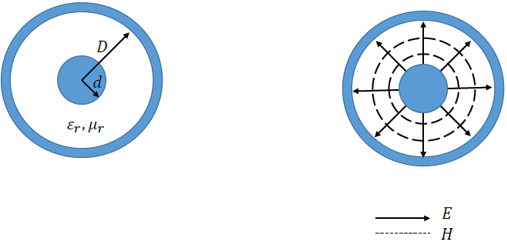
\includegraphics[width=8cm]{./images/Coax.png}
\end{minipage}
\\
\\
\\
\begin{minipage}{6cm}
	\textbf{Striplines (TEM Mode only):}\\ 
	Striplines can support TEM mode only, provided that $b<< \lambda/4$ where $\lambda$ is the wavelength in the medium.\\ \\
	$ Z_0 = \frac{30\pi}{\sqrt{\epsilon_r}}\cdot \frac{b}{W_e + 0.441\cdot b}$\\ \\
\end{minipage}
\hspace{4cm}
\begin{minipage}{8cm}
	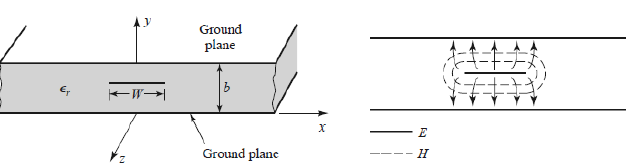
\includegraphics[width=8cm]{./images/Stripline.png}
\end{minipage}
\\
\\
\\
\\
\begin{minipage}{6cm}
	\textbf{Micro Striplines (TEM Mode only):}\\ 
	To keep the equations (field distribution) simpler  $y > d$\\
	\\
	$Z_0 =\begin{cases}&\text{$\frac{60}{\sqrt{\epsilon_e}}\ln (\frac{8d}{W}+\frac{W}{4d})$ $\hspace{3cm}$ for $ W/d \leq 1 $}\\&\text{$\frac{120\pi}{\sqrt{\epsilon_e}\cdot [W/d + 1.393 + 0.667 \ln(W/d+1.44)]} \hspace{1cm}$ for $ W/d \geq 1 $ }\end{cases}$ \\
	\\
	where $\epsilon_e$ is:\\
	\\
	$\epsilon_e \approx \frac{\epsilon_r+1}{2}+\frac{\epsilon_r-1}{2}\cdot \frac{1}{\sqrt{1+10\frac{d}{W}}}$
	
	
\end{minipage}
\hspace{4cm}
\begin{minipage}{8cm}
	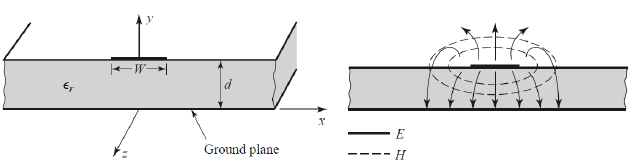
\includegraphics[width=8cm]{./images/MicroStripline.png}
\end{minipage}

\newpage